\documentclass[a4paper,10pt]{article}
\usepackage[english]{babel}
\usepackage[utf8]{inputenc}
\usepackage[toc,page]{appendix}
\usepackage{graphicx}
\usepackage{multirow}
\usepackage{array}

%Includes "References" in the table of contents
\usepackage[nottoc]{tocbibind}
\usepackage{titling}
\usepackage{setspace}




\parskip .8ex

%\setlength{\droptitle}{-10em}
\setlength{\topmargin}{-0.5in} % was -1

\usepackage{fancyheadings}
\usepackage{ifthen}
\usepackage{titlesec}
\setlength{\textheight}{9.5in} %was 10.2

%Begining of the document
\begin{document}

\title{\textbf{CSCM35: Big Data and Data Mining \\Coursework 2}}
\date{01/05/20}
\author{Andy Gray\\445348}



% Build the title and declaration pages, and pad the document so the text starts on a right hand book page.
% Page numbering is in roman numerals until the first page of an actual chapter which resets numbers 
% starting from 1 at that point. 

%\begin{figure}[t]
%	
\includegraphics[width=8cm]{swansea.png}
%	\centering
%\end{figure}
\maketitle
\begin{center}
\item
\includegraphics[width=9cm]{swansea.png}
\end{center}

\thispagestyle{empty}
\newpage
\pagenumbering{arabic}

\section{Introduction}

%\small 
We have presented upon us a challenge to complete a practical data mining task, which involves a technical report and a software solution. We have a dataset provided that has been collect by Johns Hopkins CSSE in real-time, with values related to the current pandemic the coronavirus (COVID-19). However, we need to use additional datasets to complete complement the provided data. Once identifying a research question, we need to develop a prototype and evaluate our method. 

With the COVID-19 first declaring over 800 cases on the 23rd of January 2020, and figures still rising, which at point of writing was 3.12m cases and 217K deaths worldwide \cite{worldmeter}, the virus has reached over 199 different countries. We wanted to see if between the time scale of the 22nd of January and the 25th of April, what is the general public sentiment is. We want to know, has the general public sentiment changed, or if it has stayed the same? While over the COVID-19 pandemic.

We will first achieve this by using Twitters API to gain all the tweets that have been tweeted, over this time, using the hashtag 'coronavirus'. We will then complete a sentiment analysis on the data, to gain an overall view of the general feel of the 'coronavirus' tweets. Gaining the sentiment value will allow us to have insights into the public view, and if these tweets are positive, neutral or negative and how they change as the pandemic plays out over time. 

[Overview of the results here]

[Overview of what to expect in the document]

\section{Proposed Solution}
We will be using twarc, a Python library for archiving Twitter JSON data. The library accesses the Twitter API to extract a JSON object as Twitter stores tweets as line-oriented JSON. The twarc library handles the Twitters's API, as well, as its rate limits. This library also allows us to use hydrate tweet ids. It is collecting the relevant tweet's details that match the criteria of having hashtags of 'coronavirus', 'virus', 'covid'.

We will then use another python library called hydrate. Hydrate [explain it]. Once the tweets get collected for all of the Tweet IDs, we will then convert the JSON data into a CSV file. We will then do sentiment analysis on the tweets to gauge the over feel of these tweets. To see if they are all negative, neutral or if they overall a positive vibe over each day.

[Need to explain the stages after this as this is where I am in the practicle]

We will then use NLTK to create a sentiment analysis on the tweets text body. [Explain what we did in stages]

We will then use the ARIMA algorithm to predict where we think the general mood about the COVID-19 on twitter is heading, more into a negative direction, or is it neutral or moving into a positive direction.



\subsection{Packages}
%Need to update.
We will be using the programming language Python 3 \cite{Python}, as this allows us to use all the required additional packages needed. The additional packages we will be using are NumPy \cite{walt2011numpy}, OpenCV \cite{opencv_library}, Pptk, Matplotlib \cite{hunter2007matplotlib}, SKImages \cite{van2014scikit}, SKLearn \cite{sklearn_api} and Tensorflow version 2 \cite{tensorflow2015-whitepaper}.

\subsection{Dataset}
The presented dataset provided, which is maintained by Johns Hopkins CSSE, consists of [decsribe data here]. The data had many missing values, which correlate to the country not having any COVID-19 cases, so these features got filled in with zeros.

With using Twarc, we were able to gain 15million tweets.

\subsection{Sentiment Analysis}
Sentiment analysis is a type of data mining. It aims to measure what the inclination of people's opinions is, through using natural language processing (NLP). NLP is a computational linguistics and text analysis. It gets used to extract and analyse information from the Web, which is mostly social media and other similar sources. The analysed data quantifies the general public's sentiments or reactions toward certain situations, products, people or ideas and reveal the contextual polarity of the information. Sentiment analysis is also known as opinion mining \cite{towarddatasciencesentiment}.

Sentiment analysis can fall into two categories, pure statistics or a mix of statistics and linguistics \cite{towarddatasciencesentiment}. Pure statistics use algorithms like the Bag of Words (BOW). This kind of algorithms filters the text down to only the words that the algorithm believes to have sentiment, taking into account no context to the sentence at all. Such models do not aim to understand the language, only analyse the statistical measures to classify the text. [Will I use this approach?] 

The mix of statistics and linguistics approach uses an array of Natural Language Processing (NLP) techniques, along with statistics to allow the machine to understand the language truly. The algorithms achieve this by incorporating languages grammar principles into analyst of the text. 

There are broadly two main outputs to sentiment analysis. One type of sentiment analysis output gets referred to as Categorical/Polarity. What this means is that the text will get classed as either positive, negative or neutral overall. While the other is Scalar/Degree. What this means is that a score is given based on a predefined scale, that ranges from highly positive to highly negative. This type of sentiment analysis output has been used on tweets to see the views on various USA election candidates.

\subsubsection{NLTK}
% This is part of the sentiment analysis??


\subsubsection{ARIMA}
% Explain this algorithm?


\subsection{Analysis Tools}
% This section might not be needed. Just add into packages used. ?? Maybe?

%\subsection{Visual and Statistical Analysis}

\section{Results}

%\begin{figure}[t]
%	\label{confusion_matrix}
%	\small
%	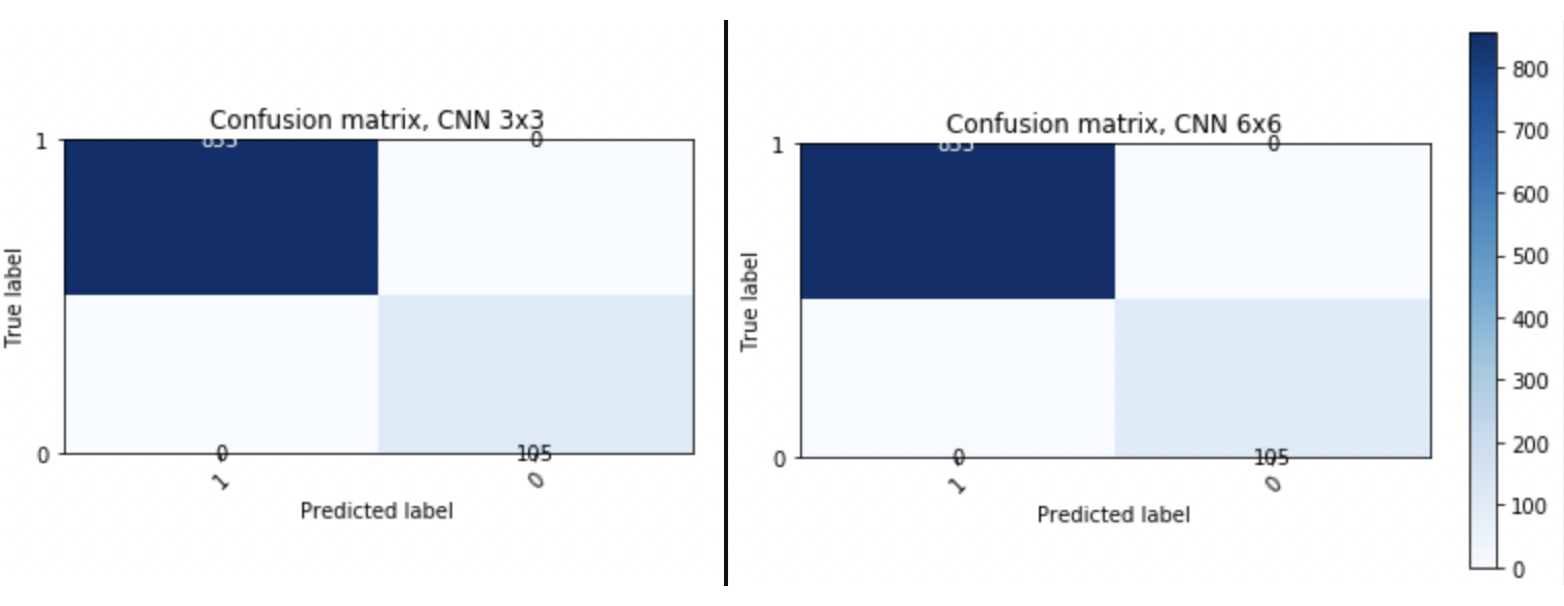
\includegraphics[width=8cm]{confusion_matrix.png}
%	\\Fig \ref{confusion_matrix}: This is the confusion matrix from the 3x3 and 6x6 filter training.
%	\centering
%\end{figure}

%\begin{center}
%	\label{confusion_matrix}
%	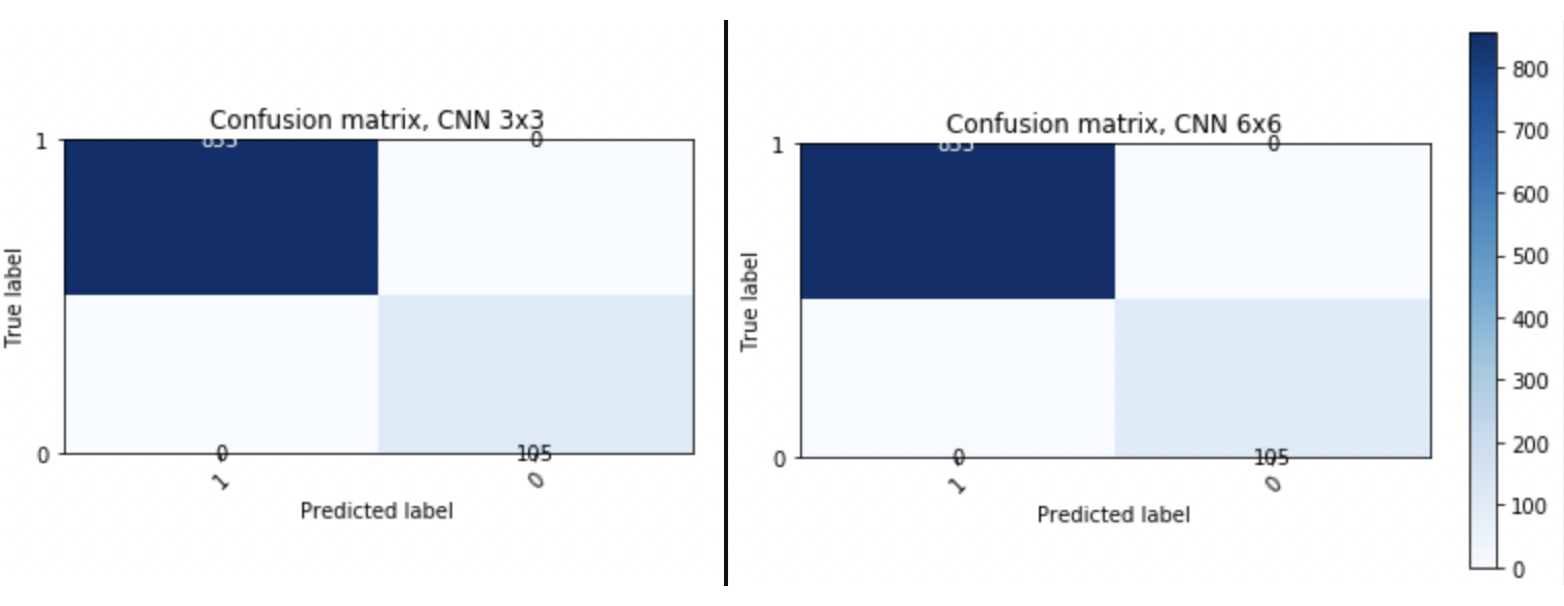
\includegraphics[width=8cm]{confusion_matrix.png}
%\end{center}


%\begin{center}
%	\begin{tabular}{ |c|p{1.5cm}|p{2.25cm}|p{2.25cm}|p{2.25cm}| } 
		
%		\hline
%		 & CCN Taining Time & 2 Step Sliding Window & 5 Step Sliding Window & 10 Step Sliding Window \\
%		\hline
%		\multirow{3}{4em}{3x3 Filter} & 6.91 sec & 708.19 sec & 716.51 sec & 1060.81 sec \\ 
		
%		& 7.11 sec & 860.16 sec & 861.87 sec & 881.87 sec  \\ 
%		& 6.50 sec & 637.75 sec & 641.66 sec & 856.81 sec \\ 
%		\hline
%		\multirow{3}{4em}{6x6 Filter} & 9.85 sec & 1486.03 sec & 767.54 sec & 783.68 sec \\ 
%		& 11.65 sec & 1035.58 sec & 909.84 sec & 881.36 sec \\ 
%		& 9.35 sec & 757.05 sec & 753.31 sec & 955.60 sec \\ 
%		\hline
%	\end{tabular}
%\end{center}


\section{Discussion}


\section{Conclusion}




%\medskip
\newpage
%\begin{appendices}
%	\section{Total count for Country}
%	\label{appendix:totalcountall}
%	%% Add image of graph here.
%	%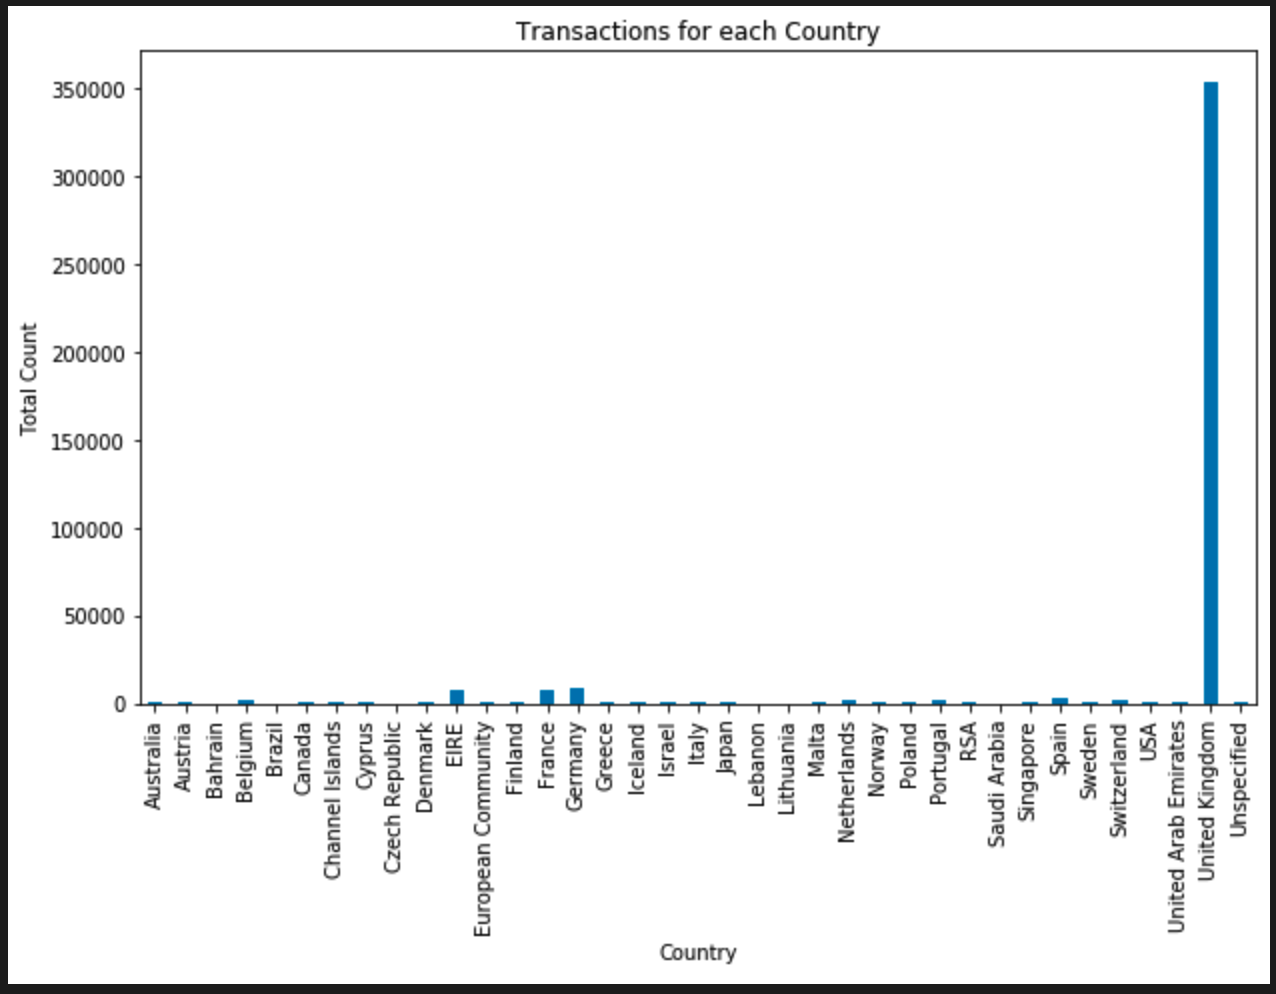
\includegraphics[scale=0.5]{totalcount}
%	
%	\section{Lift Table of Items Whole Dataset}
%	\label{appendix:wholelift}
%	%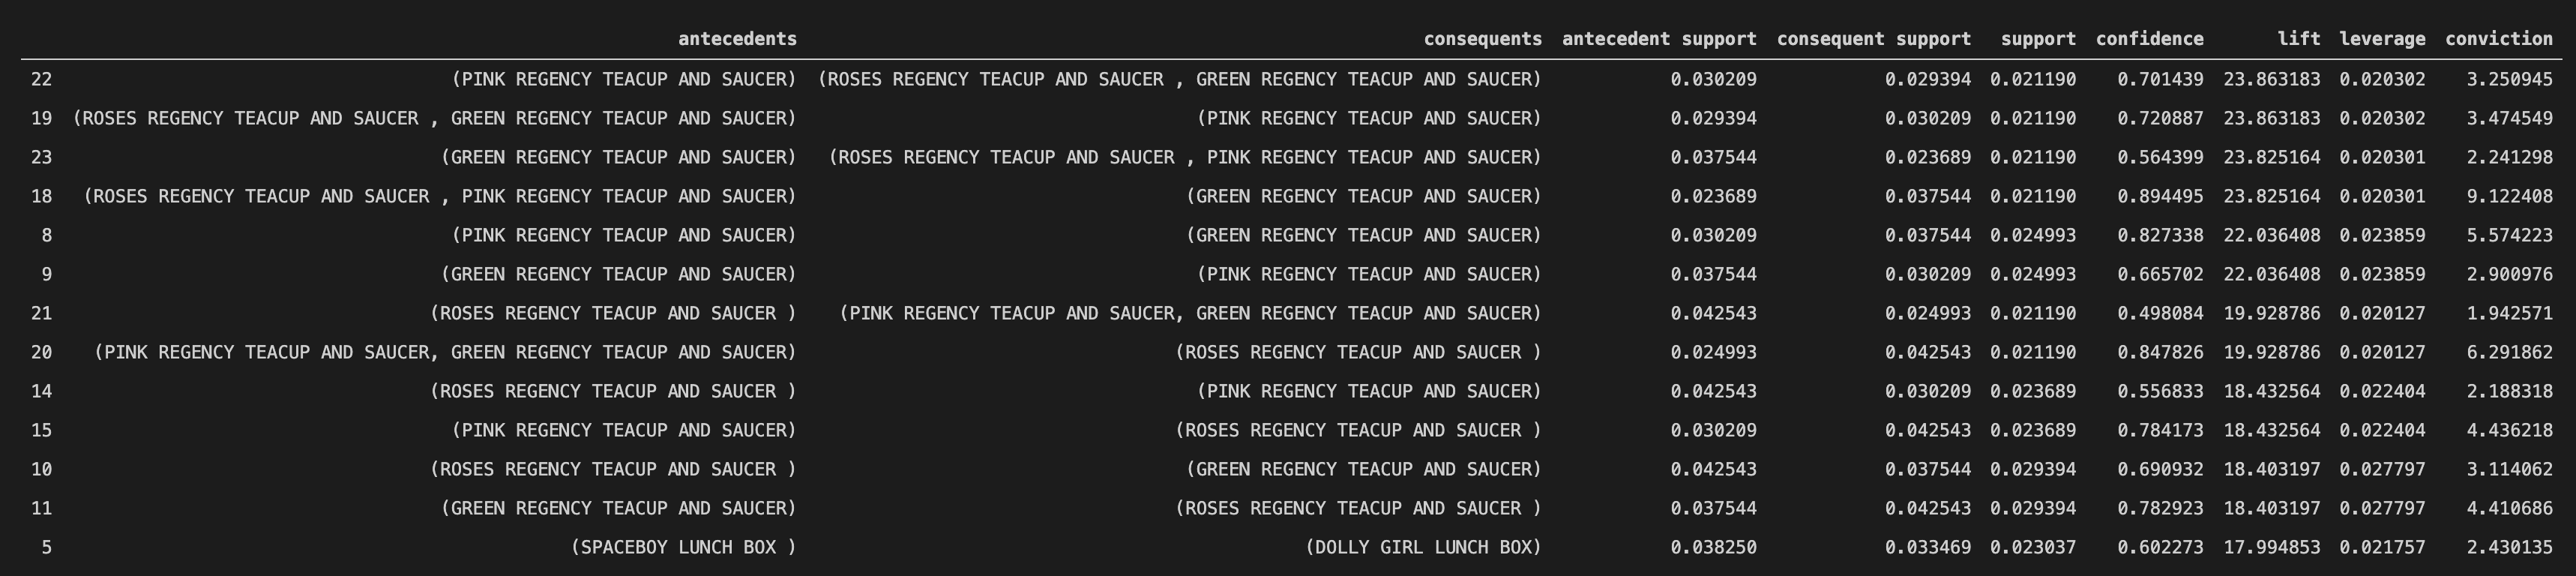
\includegraphics[scale=0.2]{wholelift}

%	\section{Confidence Table of Items Whole Dataset}
%	\label{appendix:wholeconf}
	%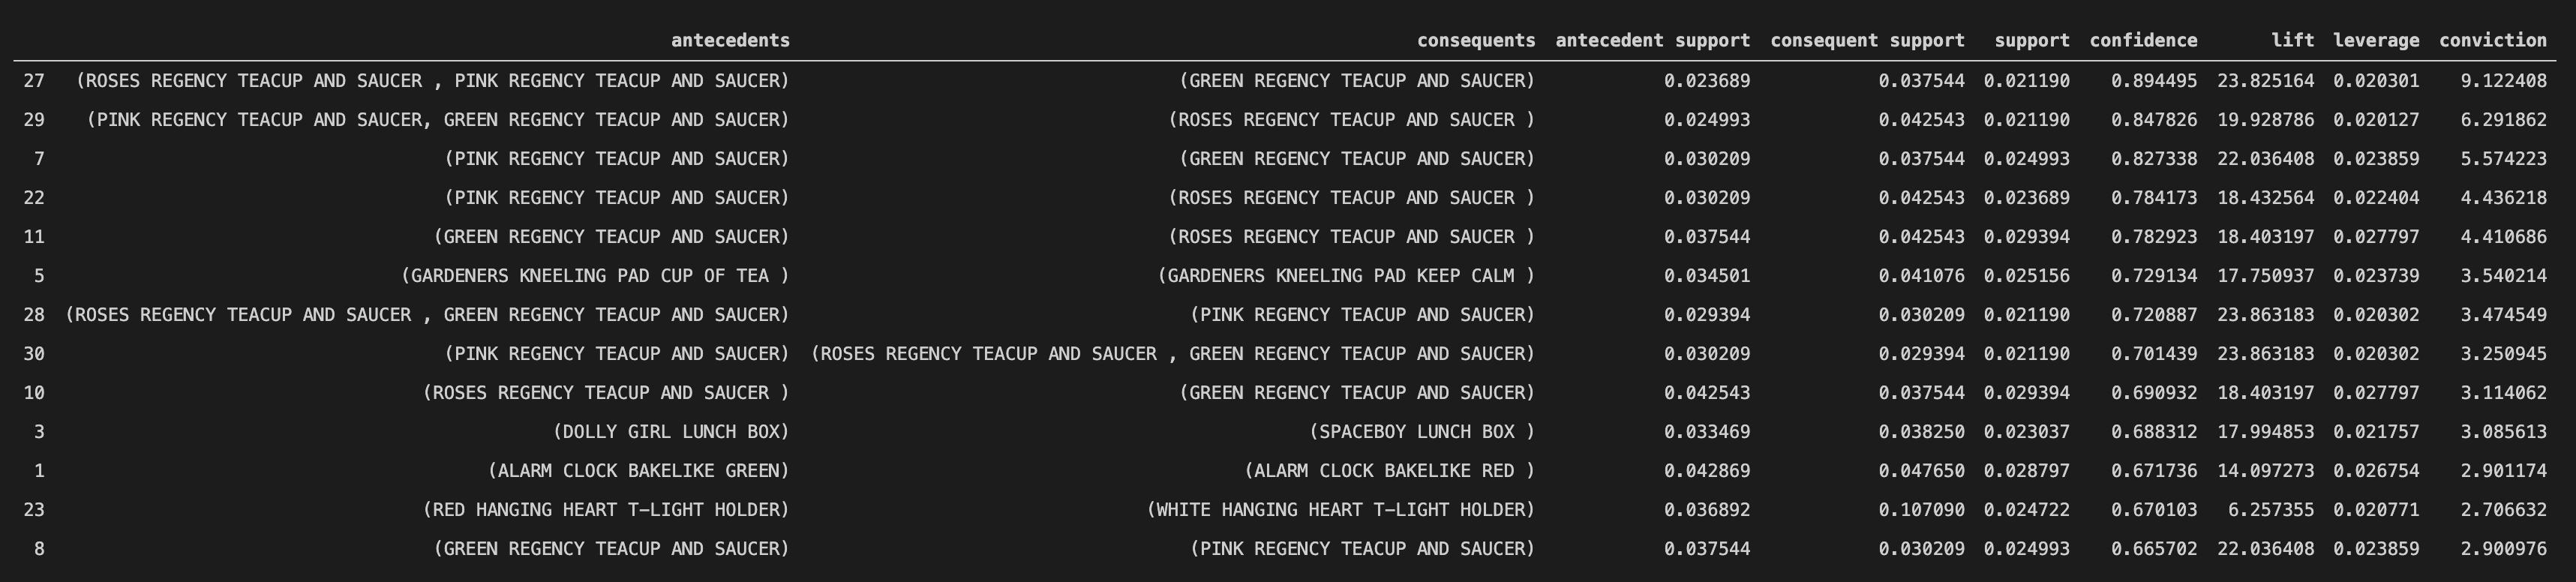
\includegraphics[scale=0.2]{wholeconf}
	
%	\section{Lift Table of United Kingdom Items}
%	\label{appendix:uklift}
	%% Add image of graph here.
	%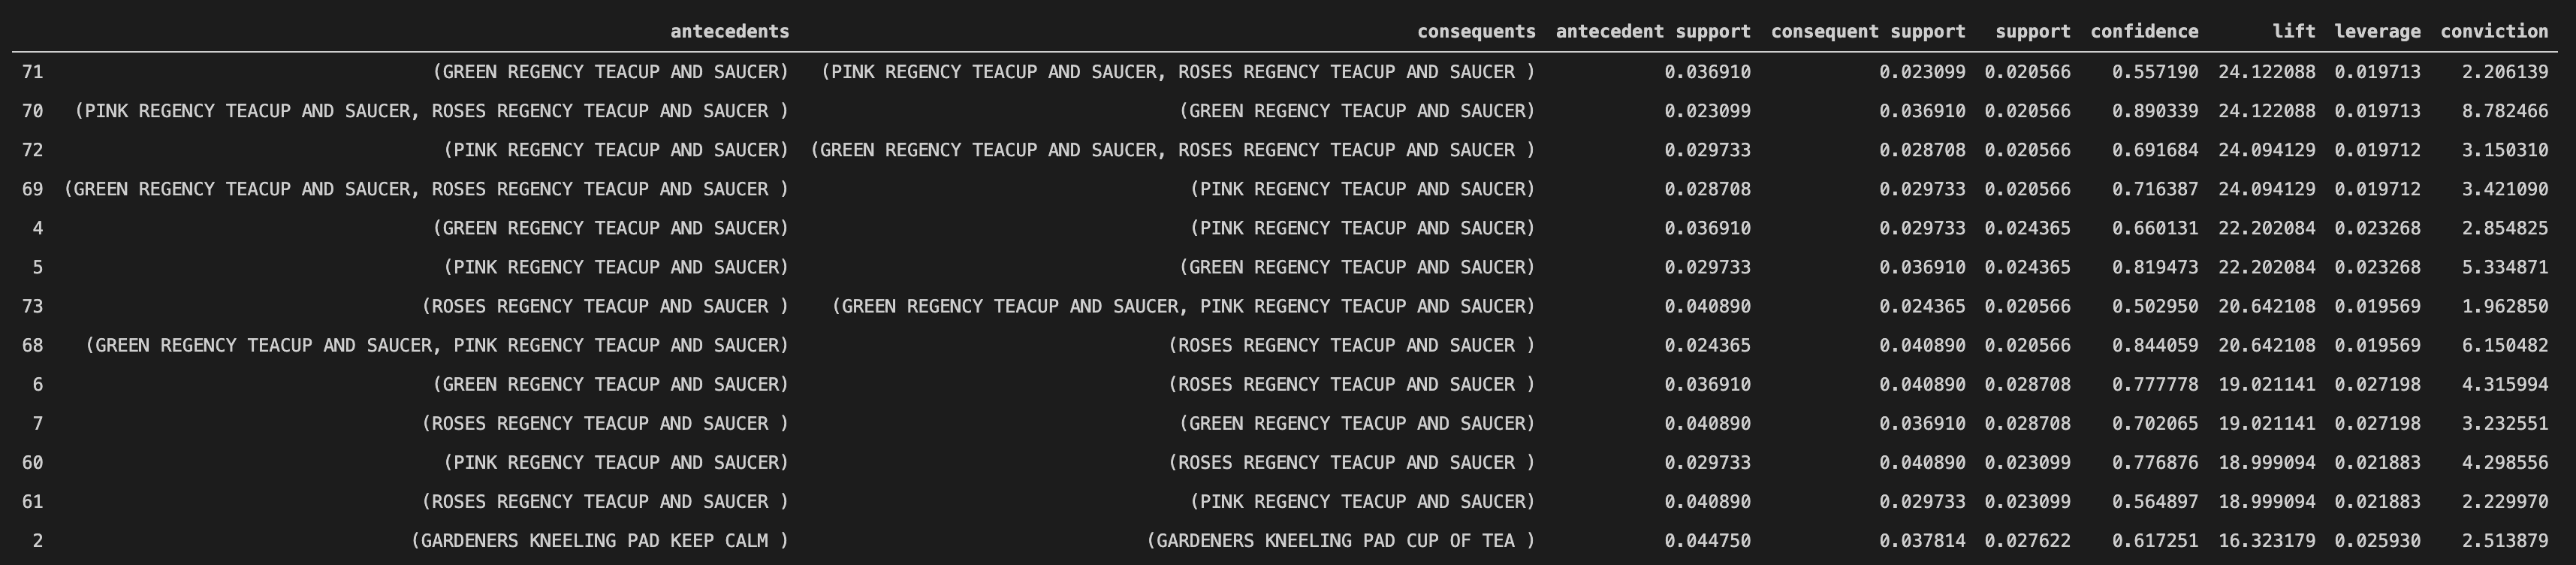
\includegraphics[scale=0.2]{uklift}
	
%	\section{Confidence Table of United Kingdom Items}
%	\label{appendix:ukconf}
	%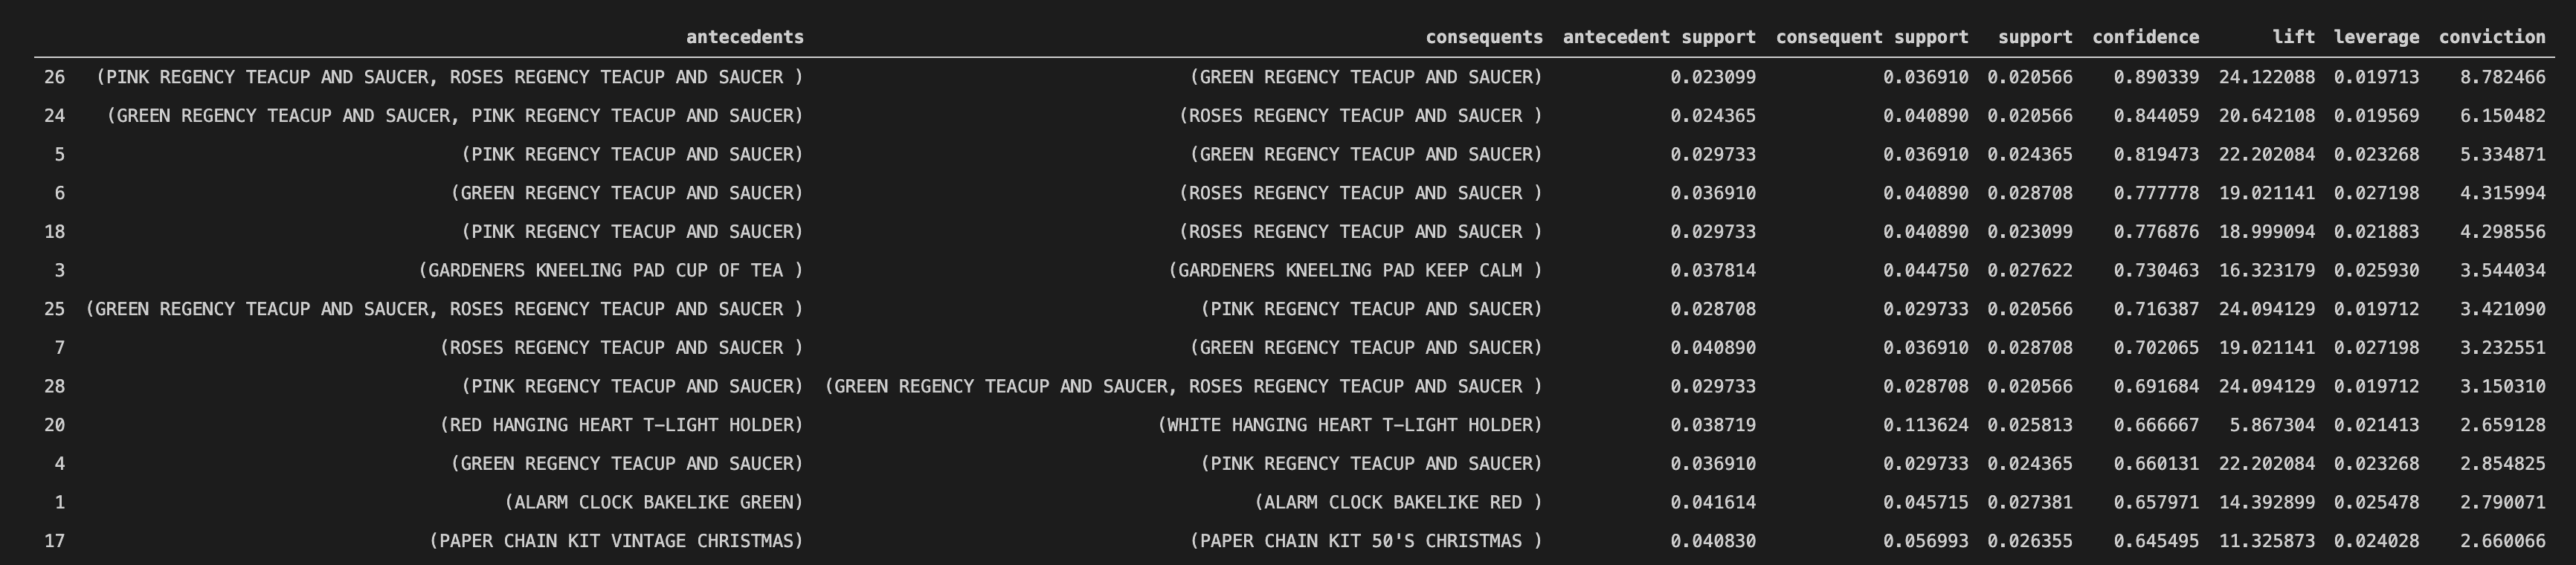
\includegraphics[scale=0.2]{ukconf}
	
%	\section{Lift Table of Germany Items}
%	\label{appendix:germanylift}
	%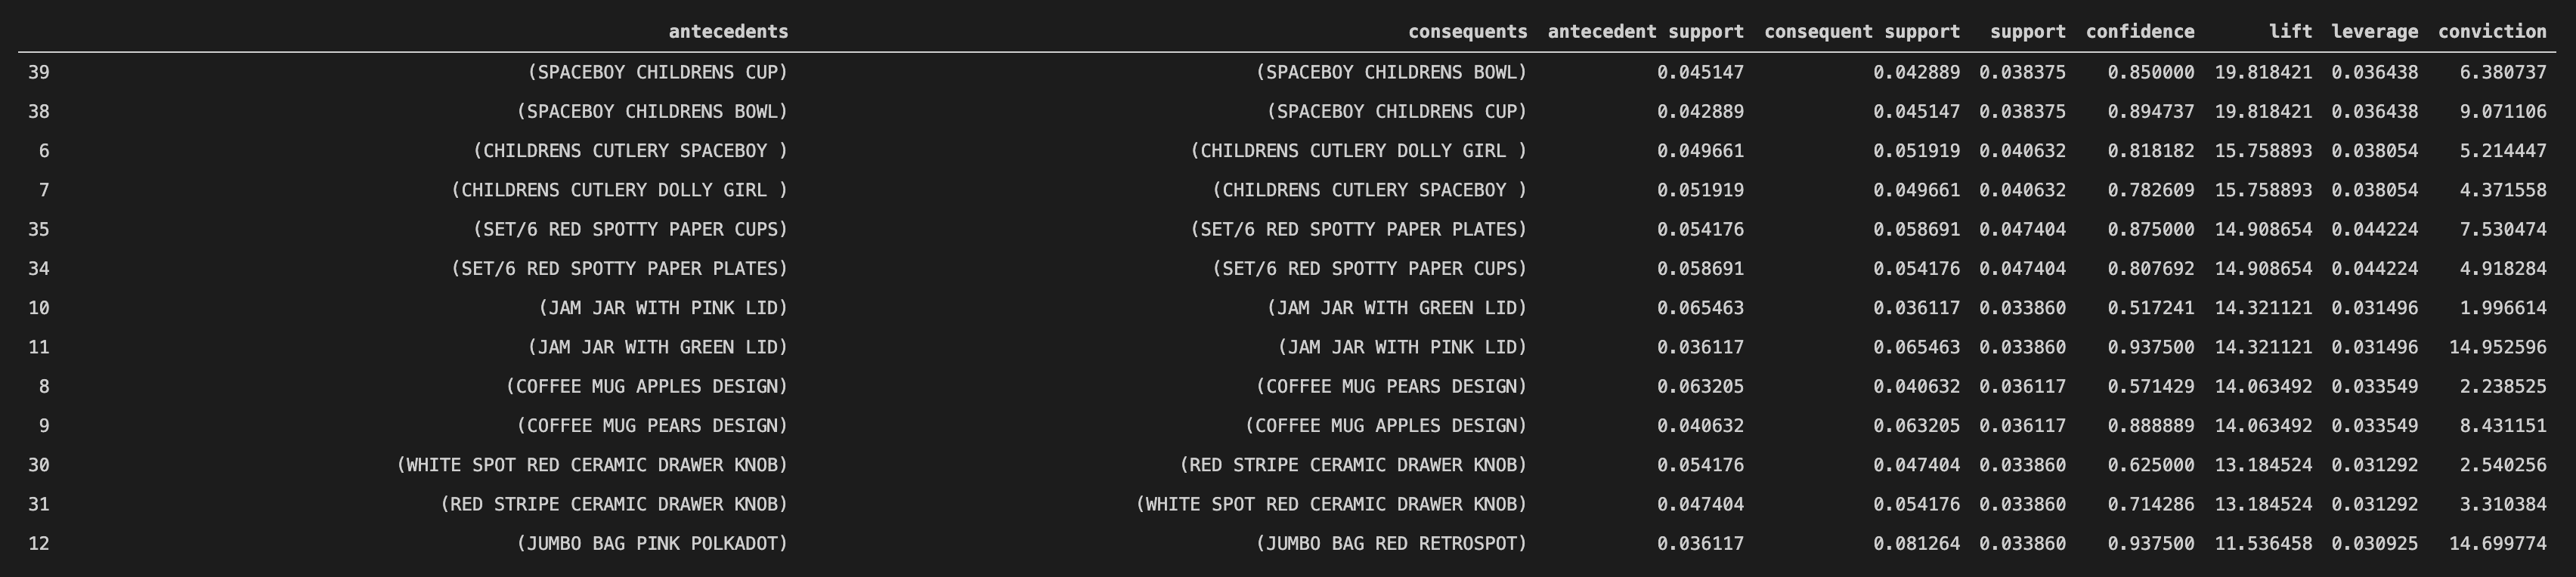
\includegraphics[scale=0.2]{germanylift}
	
%	\section{Confidence Table of Germany Items}
%	\label{appendix:germanyconf}
	%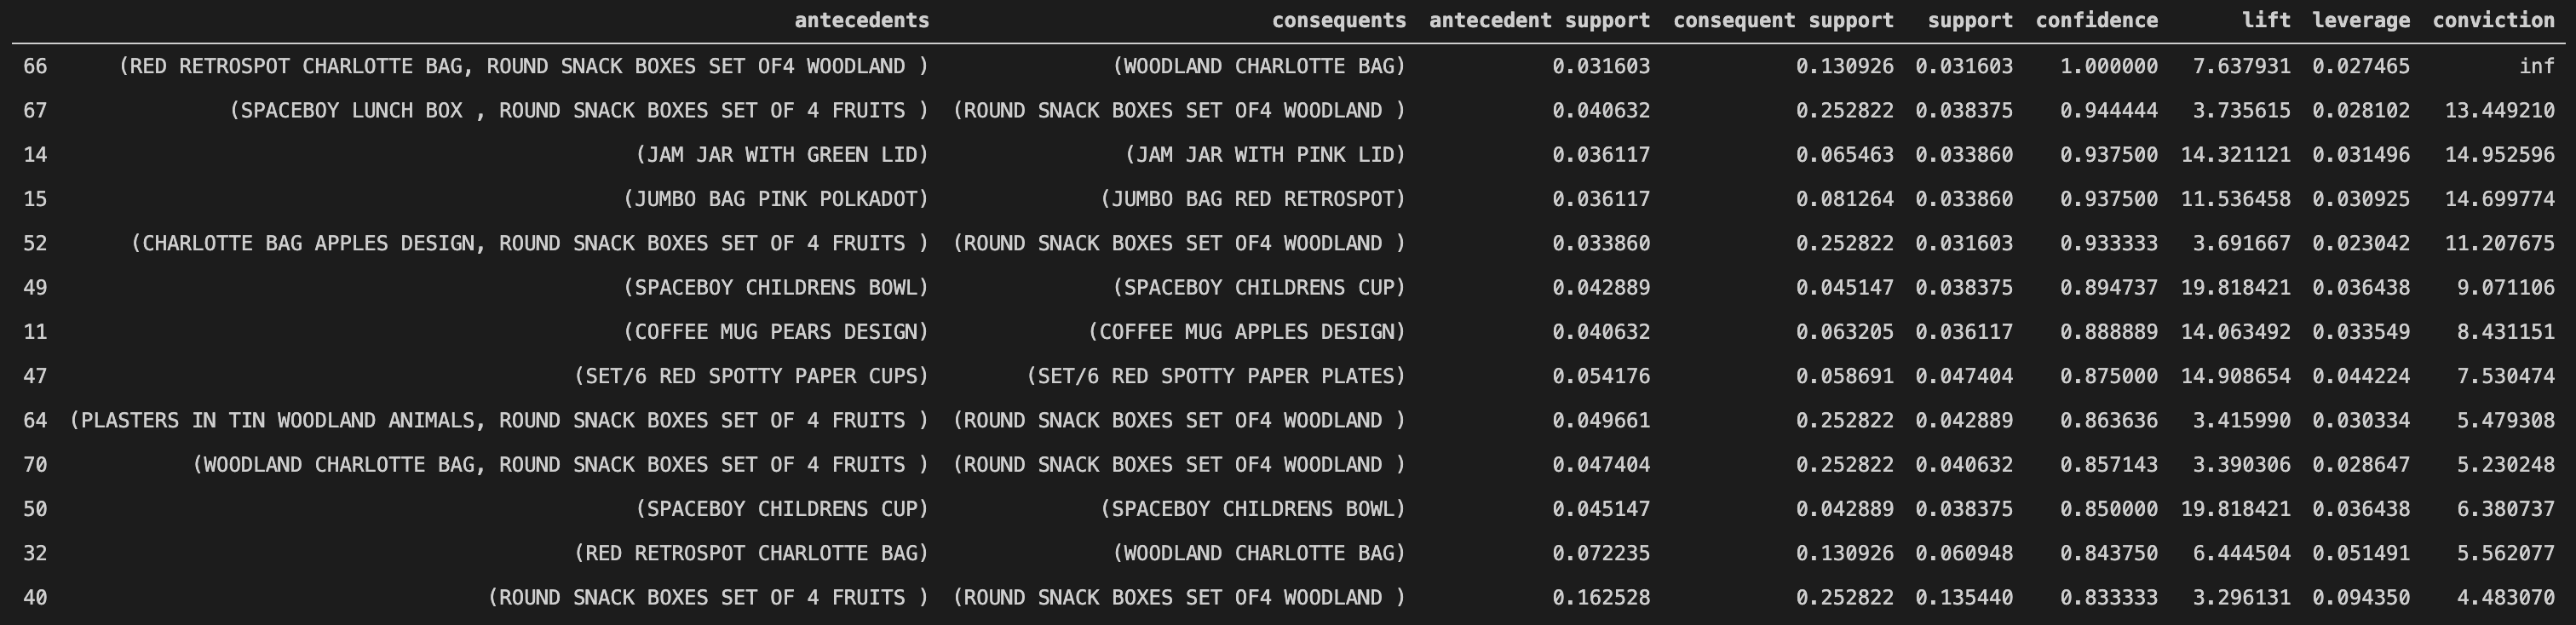
\includegraphics[scale=0.2]{germanyconf}
	
%	\section{Lift Table of France Items}
%	\label{appendix:francelift}
	%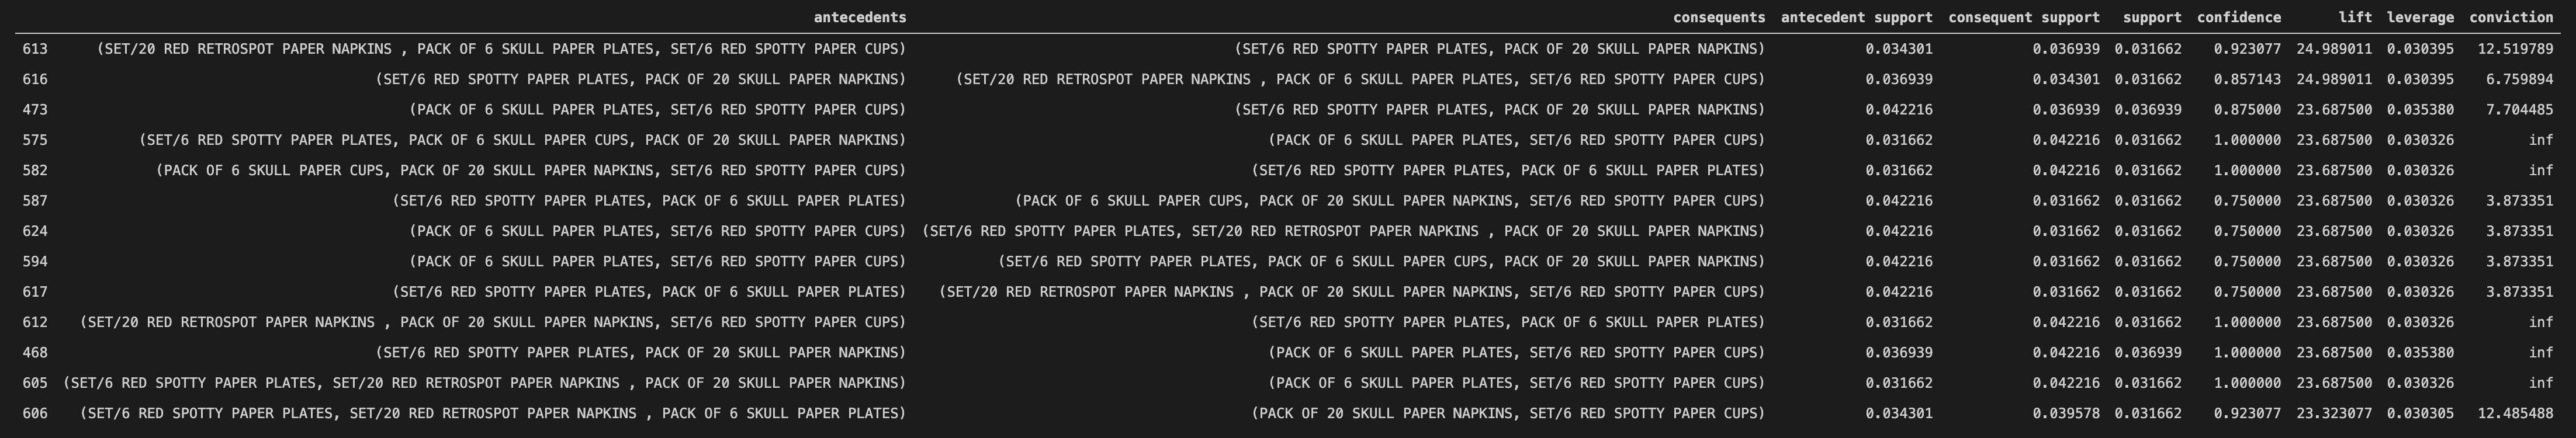
\includegraphics[scale=0.2]{francelift}
	
%	\section{Confidence Table of France Items}
%	\label{appendix:franceconf}
	%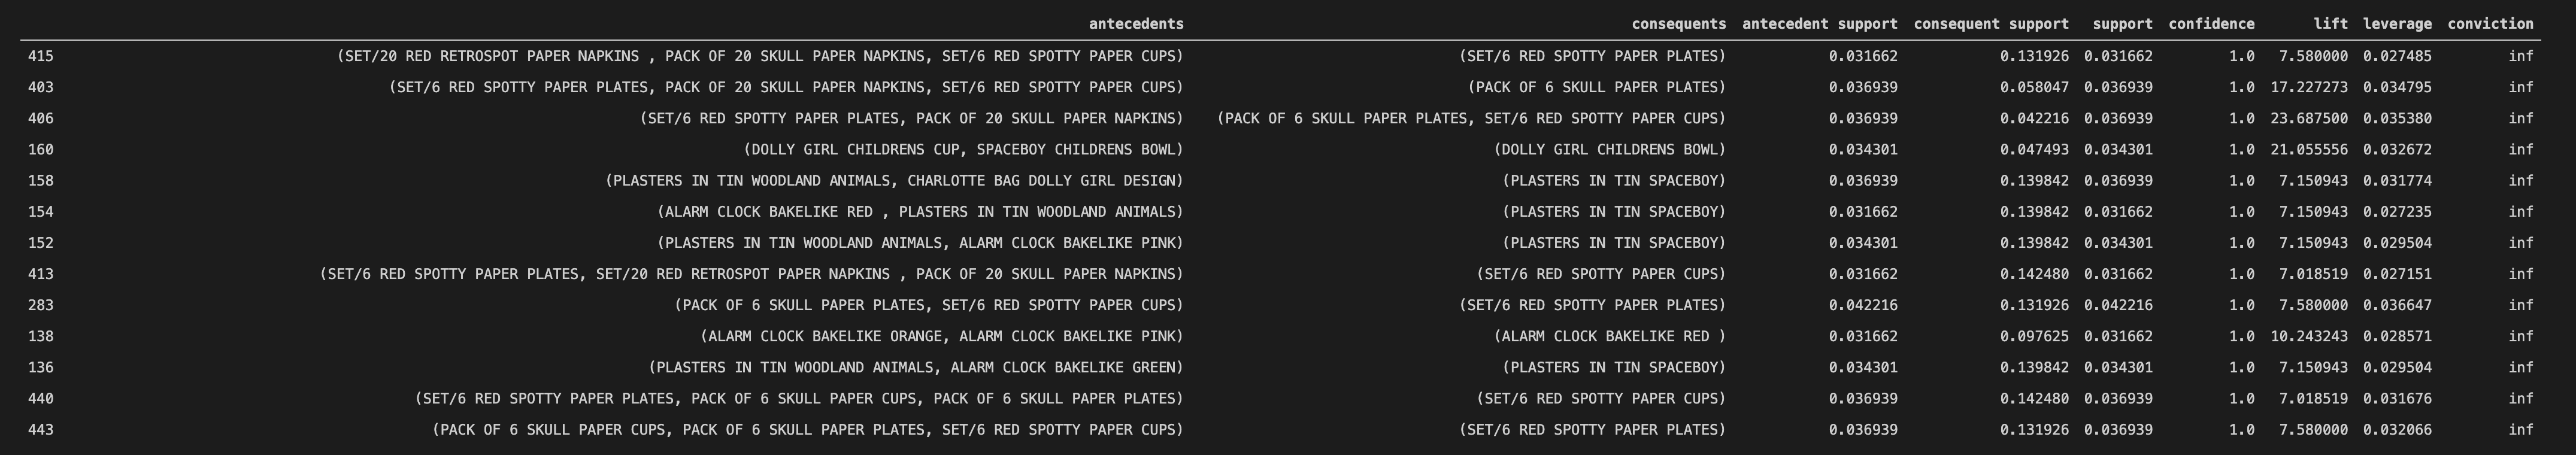
\includegraphics[scale=0.2]{franceconf}
	
%	\section{Lift Table of Erie Items}
%	\label{appendix:eirelift}
	%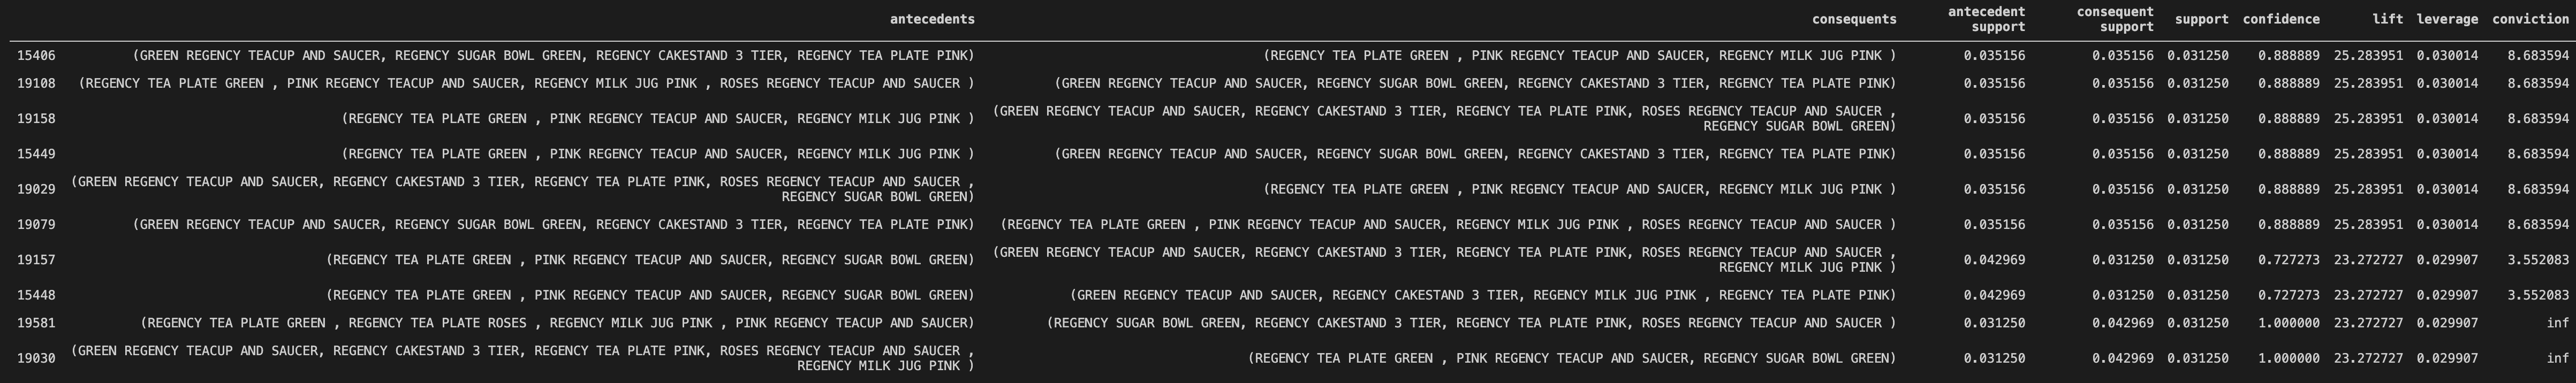
\includegraphics[scale=0.19]{eirelift}
	
%	\section{Confidence Table of Eire Items}
%	\label{appendix:eireconf}
	%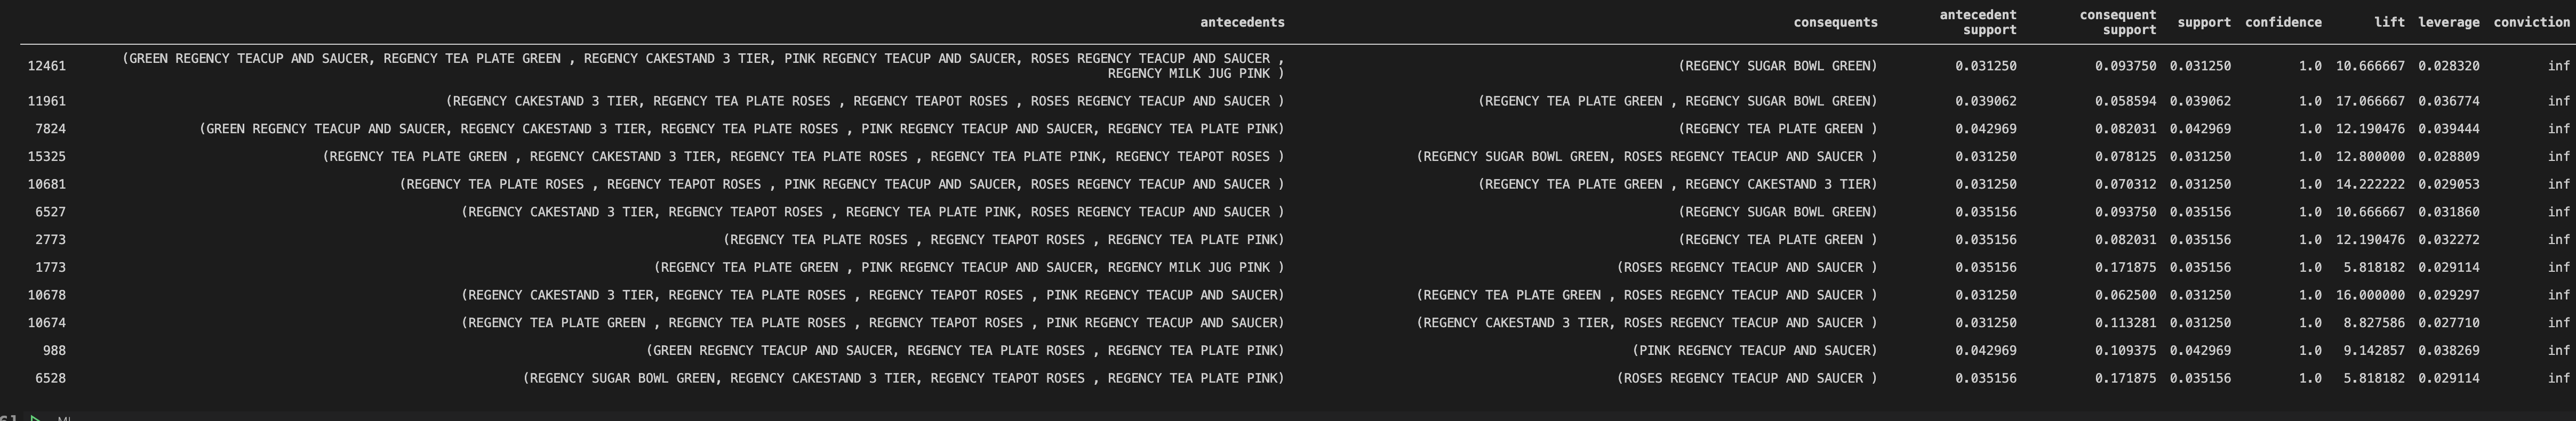
\includegraphics[scale=0.19]{eireconf}
	
%\end{appendices}

%\newpage

%Sets the bibliography style to UNSRT and imports the 
%bibliography file "samples.bib".
\bibliographystyle{acm}

{\footnotesize
	\bibliography{samples}
}


\end{document}